\documentclass[11pt,compress,t,notes=noshow, xcolor=table]{beamer}
\usepackage[]{graphicx}\usepackage[]{color}
% maxwidth is the original width if it is less than linewidth
% otherwise use linewidth (to make sure the graphics do not exceed the margin)
\makeatletter
\def\maxwidth{ %
  \ifdim\Gin@nat@width>\linewidth
    \linewidth
  \else
    \Gin@nat@width
  \fi
}
\makeatother

\definecolor{fgcolor}{rgb}{0.345, 0.345, 0.345}
\newcommand{\hlnum}[1]{\textcolor[rgb]{0.686,0.059,0.569}{#1}}%
\newcommand{\hlstr}[1]{\textcolor[rgb]{0.192,0.494,0.8}{#1}}%
\newcommand{\hlcom}[1]{\textcolor[rgb]{0.678,0.584,0.686}{\textit{#1}}}%
\newcommand{\hlopt}[1]{\textcolor[rgb]{0,0,0}{#1}}%
\newcommand{\hlstd}[1]{\textcolor[rgb]{0.345,0.345,0.345}{#1}}%
\newcommand{\hlkwa}[1]{\textcolor[rgb]{0.161,0.373,0.58}{\textbf{#1}}}%
\newcommand{\hlkwb}[1]{\textcolor[rgb]{0.69,0.353,0.396}{#1}}%
\newcommand{\hlkwc}[1]{\textcolor[rgb]{0.333,0.667,0.333}{#1}}%
\newcommand{\hlkwd}[1]{\textcolor[rgb]{0.737,0.353,0.396}{\textbf{#1}}}%
\let\hlipl\hlkwb

\usepackage{framed}
\makeatletter
\newenvironment{kframe}{%
 \def\at@end@of@kframe{}%
 \ifinner\ifhmode%
  \def\at@end@of@kframe{\end{minipage}}%
  \begin{minipage}{\columnwidth}%
 \fi\fi%
 \def\FrameCommand##1{\hskip\@totalleftmargin \hskip-\fboxsep
 \colorbox{shadecolor}{##1}\hskip-\fboxsep
     % There is no \\@totalrightmargin, so:
     \hskip-\linewidth \hskip-\@totalleftmargin \hskip\columnwidth}%
 \MakeFramed {\advance\hsize-\width
   \@totalleftmargin\z@ \linewidth\hsize
   \@setminipage}}%
 {\par\unskip\endMakeFramed%
 \at@end@of@kframe}
\makeatother

\definecolor{shadecolor}{rgb}{.97, .97, .97}
\definecolor{messagecolor}{rgb}{0, 0, 0}
\definecolor{warningcolor}{rgb}{1, 0, 1}
\definecolor{errorcolor}{rgb}{1, 0, 0}
\newenvironment{knitrout}{}{} % an empty environment to be redefined in TeX

\usepackage{alltt}
\newcommand{\SweaveOpts}[1]{}  % do not interfere with LaTeX
\newcommand{\SweaveInput}[1]{} % because they are not real TeX commands
\newcommand{\Sexpr}[1]{}       % will only be parsed by R
\newcommand{\xmark}{\ding{55}}%


\usepackage[english]{babel}
\usepackage[utf8]{inputenc}

\usepackage{dsfont}
\usepackage{verbatim}
\usepackage{amsmath}
\usepackage{amsfonts}
\usepackage{amssymb}
\usepackage{bm}
\usepackage{csquotes}
\usepackage{multirow}
\usepackage{longtable}
\usepackage{booktabs}
\usepackage{enumerate}
\usepackage[absolute,overlay]{textpos}
\usepackage{psfrag}
\usepackage{algorithm}
\usepackage{algpseudocode}
\usepackage{eqnarray}
\usepackage{arydshln}
\usepackage{tabularx}
\usepackage{placeins}
\usepackage{tikz}
\usepackage{setspace}
\usepackage{colortbl}
\usepackage{mathtools}
\usepackage{wrapfig}
\usepackage{bm}
\usepackage{amsmath}
\usepackage{pifont}
\usepackage[round]{natbib}
\usepackage{hyperref}

\usetikzlibrary{shapes,arrows,automata,positioning,calc,chains,trees, shadows}
\tikzset{
  %Define standard arrow tip
  >=stealth',
  %Define style for boxes
  punkt/.style={
    rectangle,
    rounded corners,
    draw=black, very thick,
    text width=6.5em,
    minimum height=2em,
    text centered},
  % Define arrow style
  pil/.style={
    ->,
    thick,
    shorten <=2pt,
    shorten >=2pt,}
}

\usepackage{subfig}

% Defines macros and environments
\usepackage{../../style/lmu-lecture}


\let\code=\texttt
\let\proglang=\textsf

\setkeys{Gin}{width=0.9\textwidth}

\setbeamertemplate{frametitle}{\expandafter\uppercase\expandafter\insertframetitle}

% basic latex stuff
\newcommand{\pkg}[1]{{\fontseries{b}\selectfont #1}} % fontstyle for R packages

% Often used in exercise Rnw files, still relevant?
\newcommand{\lz}{\vspace{0.5cm}} % vertical space
\newcommand{\dlz}{\vspace{1cm}}  % double vertical space

% Unused and about to be deleted
\newcommand{\oneliner}[1] % Oneliner for important statements
{\begin{block}{}\begin{center}\begin{Large}#1\end{Large}\end{center}\end{block}}


%--------------------%
%  New environments  %
%--------------------%

 % Frame with breaks and verbatim // this is used very often
\newenvironment{vbframe}
{
\begin{frame}[containsverbatim,allowframebreaks]
}
{
\end{frame}
}

% Frame with verbatim without breaks (to avoid numbering one slided frames)
% This is not used anywhere but I can see it being useful
\newenvironment{vframe}
{
\begin{frame}[containsverbatim]
}
{
\end{frame}
}

% Itemize block
\newenvironment{blocki}[1]
{
\begin{block}{#1}\begin{itemize}
}
{
\end{itemize}\end{block}
}

%--------------%
%  Citebutton  %
%--------------%
% Example usage (from slides-cart-discussion.tex)
% \citebutton{Breiman, 1984}{https://www.taylorfrancis.com/books/mono/10.1201/9781315139470/classification-regression-trees-leo-breiman}
\newcommand{\citebutton}[2]{%
\NoCaseChange{\resizebox{!}{9pt}{\protect\beamergotobutton{\href{#2}{#1}}}}%
}

% textcolor that works in mathmode
% https://tex.stackexchange.com/a/261480
% Used e.g. in forests/slides-forests-bagging.tex
% [...] \textcolor{blue}{\tfrac{1}{M}\sum^M_{m} [...]
\makeatletter
\renewcommand*{\@textcolor}[3]{%
  \protect\leavevmode
  \begingroup
    \color#1{#2}#3%
  \endgroup
}
\makeatother





% dependencies: amsmath, amssymb, dsfont
% math spaces
\ifdefined\N
\renewcommand{\N}{\mathds{N}} % N, naturals
\else \newcommand{\N}{\mathds{N}} \fi
\newcommand{\Z}{\mathds{Z}} % Z, integers
\newcommand{\Q}{\mathds{Q}} % Q, rationals
\newcommand{\R}{\mathds{R}} % R, reals
\ifdefined\C
\renewcommand{\C}{\mathds{C}} % C, complex
\else \newcommand{\C}{\mathds{C}} \fi
\newcommand{\continuous}{\mathcal{C}} % C, space of continuous functions
\newcommand{\M}{\mathcal{M}} % machine numbers
\newcommand{\epsm}{\epsilon_m} % maximum error

% counting / finite sets
\newcommand{\setzo}{\{0, 1\}} % set 0, 1
\newcommand{\setmp}{\{-1, +1\}} % set -1, 1
\newcommand{\unitint}{[0, 1]} % unit interval

% basic math stuff
\newcommand{\xt}{\tilde x} % x tilde
\DeclareMathOperator*{\argmax}{arg\,max} % argmax
\DeclareMathOperator*{\argmin}{arg\,min} % argmin
\newcommand{\argminlim}{\mathop{\mathrm{arg\,min}}\limits} % argmax with limits
\newcommand{\argmaxlim}{\mathop{\mathrm{arg\,max}}\limits} % argmin with limits
\newcommand{\sign}{\operatorname{sign}} % sign, signum
\newcommand{\I}{\mathbb{I}} % I, indicator
\newcommand{\order}{\mathcal{O}} % O, order
\newcommand{\bigO}{\mathcal{O}} % Big-O Landau
\newcommand{\littleo}{{o}} % Little-o Landau
\newcommand{\pd}[2]{\frac{\partial{#1}}{\partial #2}} % partial derivative
\newcommand{\floorlr}[1]{\left\lfloor #1 \right\rfloor} % floor
\newcommand{\ceillr}[1]{\left\lceil #1 \right\rceil} % ceiling
\newcommand{\indep}{\perp \!\!\! \perp} % independence symbol

% sums and products
\newcommand{\sumin}{\sum\limits_{i=1}^n} % summation from i=1 to n
\newcommand{\sumim}{\sum\limits_{i=1}^m} % summation from i=1 to m
\newcommand{\sumjn}{\sum\limits_{j=1}^n} % summation from j=1 to p
\newcommand{\sumjp}{\sum\limits_{j=1}^p} % summation from j=1 to p
\newcommand{\sumik}{\sum\limits_{i=1}^k} % summation from i=1 to k
\newcommand{\sumkg}{\sum\limits_{k=1}^g} % summation from k=1 to g
\newcommand{\sumjg}{\sum\limits_{j=1}^g} % summation from j=1 to g
\newcommand{\meanin}{\frac{1}{n} \sum\limits_{i=1}^n} % mean from i=1 to n
\newcommand{\meanim}{\frac{1}{m} \sum\limits_{i=1}^m} % mean from i=1 to n
\newcommand{\meankg}{\frac{1}{g} \sum\limits_{k=1}^g} % mean from k=1 to g
\newcommand{\prodin}{\prod\limits_{i=1}^n} % product from i=1 to n
\newcommand{\prodkg}{\prod\limits_{k=1}^g} % product from k=1 to g
\newcommand{\prodjp}{\prod\limits_{j=1}^p} % product from j=1 to p

% linear algebra
\newcommand{\one}{\bm{1}} % 1, unitvector
\newcommand{\zero}{\mathbf{0}} % 0-vector
\newcommand{\id}{\bm{I}} % I, identity
\newcommand{\diag}{\operatorname{diag}} % diag, diagonal
\newcommand{\trace}{\operatorname{tr}} % tr, trace
\newcommand{\spn}{\operatorname{span}} % span
\newcommand{\scp}[2]{\left\langle #1, #2 \right\rangle} % <.,.>, scalarproduct
\newcommand{\mat}[1]{\begin{pmatrix} #1 \end{pmatrix}} % short pmatrix command
\newcommand{\Amat}{\mathbf{A}} % matrix A
\newcommand{\Deltab}{\mathbf{\Delta}} % error term for vectors

% basic probability + stats
\renewcommand{\P}{\mathds{P}} % P, probability
\newcommand{\E}{\mathds{E}} % E, expectation
\newcommand{\var}{\mathsf{Var}} % Var, variance
\newcommand{\cov}{\mathsf{Cov}} % Cov, covariance
\newcommand{\corr}{\mathsf{Corr}} % Corr, correlation
\newcommand{\normal}{\mathcal{N}} % N of the normal distribution
\newcommand{\iid}{\overset{i.i.d}{\sim}} % dist with i.i.d superscript
\newcommand{\distas}[1]{\overset{#1}{\sim}} % ... is distributed as ...

% machine learning
\newcommand{\Xspace}{\mathcal{X}} % X, input space
\newcommand{\Yspace}{\mathcal{Y}} % Y, output space
\newcommand{\Zspace}{\mathcal{Z}} % Z, space of sampled datapoints
\newcommand{\nset}{\{1, \ldots, n\}} % set from 1 to n
\newcommand{\pset}{\{1, \ldots, p\}} % set from 1 to p
\newcommand{\gset}{\{1, \ldots, g\}} % set from 1 to g
\newcommand{\Pxy}{\mathbb{P}_{xy}} % P_xy
\newcommand{\Exy}{\mathbb{E}_{xy}} % E_xy: Expectation over random variables xy
\newcommand{\xv}{\mathbf{x}} % vector x (bold)
\newcommand{\xtil}{\tilde{\mathbf{x}}} % vector x-tilde (bold)
\newcommand{\yv}{\mathbf{y}} % vector y (bold)
\newcommand{\xy}{(\xv, y)} % observation (x, y)
\newcommand{\xvec}{\left(x_1, \ldots, x_p\right)^\top} % (x1, ..., xp)
\newcommand{\Xmat}{\mathbf{X}} % Design matrix
\newcommand{\allDatasets}{\mathds{D}} % The set of all datasets
\newcommand{\allDatasetsn}{\mathds{D}_n}  % The set of all datasets of size n
\newcommand{\D}{\mathcal{D}} % D, data
\newcommand{\Dn}{\D_n} % D_n, data of size n
\newcommand{\Dtrain}{\mathcal{D}_{\text{train}}} % D_train, training set
\newcommand{\Dtest}{\mathcal{D}_{\text{test}}} % D_test, test set
\newcommand{\xyi}[1][i]{\left(\xv^{(#1)}, y^{(#1)}\right)} % (x^i, y^i), i-th observation
\newcommand{\Dset}{\left( \xyi[1], \ldots, \xyi[n]\right)} % {(x1,y1)), ..., (xn,yn)}, data
\newcommand{\defAllDatasetsn}{(\Xspace \times \Yspace)^n} % Def. of the set of all datasets of size n
\newcommand{\defAllDatasets}{\bigcup_{n \in \N}(\Xspace \times \Yspace)^n} % Def. of the set of all datasets
\newcommand{\xdat}{\left\{ \xv^{(1)}, \ldots, \xv^{(n)}\right\}} % {x1, ..., xn}, input data
\newcommand{\ydat}{\left\{ \yv^{(1)}, \ldots, \yv^{(n)}\right\}} % {y1, ..., yn}, input data
\newcommand{\yvec}{\left(y^{(1)}, \hdots, y^{(n)}\right)^\top} % (y1, ..., yn), vector of outcomes
\newcommand{\greekxi}{\xi} % Greek letter xi
\renewcommand{\xi}[1][i]{\xv^{(#1)}} % x^i, i-th observed value of x
\newcommand{\yi}[1][i]{y^{(#1)}} % y^i, i-th observed value of y
\newcommand{\xivec}{\left(x^{(i)}_1, \ldots, x^{(i)}_p\right)^\top} % (x1^i, ..., xp^i), i-th observation vector
\newcommand{\xj}{\xv_j} % x_j, j-th feature
\newcommand{\xjvec}{\left(x^{(1)}_j, \ldots, x^{(n)}_j\right)^\top} % (x^1_j, ..., x^n_j), j-th feature vector
\newcommand{\phiv}{\mathbf{\phi}} % Basis transformation function phi
\newcommand{\phixi}{\mathbf{\phi}^{(i)}} % Basis transformation of xi: phi^i := phi(xi)

%%%%%% ml - models general
\newcommand{\lamv}{\bm{\lambda}} % lambda vector, hyperconfiguration vector
\newcommand{\Lam}{\bm{\Lambda}}	 % Lambda, space of all hpos
% Inducer / Inducing algorithm
\newcommand{\preimageInducer}{\left(\defAllDatasets\right)\times\Lam} % Set of all datasets times the hyperparameter space
\newcommand{\preimageInducerShort}{\allDatasets\times\Lam} % Set of all datasets times the hyperparameter space
% Inducer / Inducing algorithm
\newcommand{\ind}{\mathcal{I}} % Inducer, inducing algorithm, learning algorithm

% continuous prediction function f
\newcommand{\ftrue}{f_{\text{true}}}  % True underlying function (if a statistical model is assumed)
\newcommand{\ftruex}{\ftrue(\xv)} % True underlying function (if a statistical model is assumed)
\newcommand{\fx}{f(\xv)} % f(x), continuous prediction function
\newcommand{\fdomains}{f: \Xspace \rightarrow \R^g} % f with domain and co-domain
\newcommand{\Hspace}{\mathcal{H}} % hypothesis space where f is from
\newcommand{\fbayes}{f^{\ast}} % Bayes-optimal model
\newcommand{\fxbayes}{f^{\ast}(\xv)} % Bayes-optimal model
\newcommand{\fkx}[1][k]{f_{#1}(\xv)} % f_j(x), discriminant component function
\newcommand{\fh}{\hat{f}} % f hat, estimated prediction function
\newcommand{\fxh}{\fh(\xv)} % fhat(x)
\newcommand{\fxt}{f(\xv ~|~ \thetav)} % f(x | theta)
\newcommand{\fxi}{f\left(\xv^{(i)}\right)} % f(x^(i))
\newcommand{\fxih}{\hat{f}\left(\xv^{(i)}\right)} % f(x^(i))
\newcommand{\fxit}{f\left(\xv^{(i)} ~|~ \thetav\right)} % f(x^(i) | theta)
\newcommand{\fhD}{\fh_{\D}} % fhat_D, estimate of f based on D
\newcommand{\fhDtrain}{\fh_{\Dtrain}} % fhat_Dtrain, estimate of f based on D
\newcommand{\fhDnlam}{\fh_{\Dn, \lamv}} %model learned on Dn with hp lambda
\newcommand{\fhDlam}{\fh_{\D, \lamv}} %model learned on D with hp lambda
\newcommand{\fhDnlams}{\fh_{\Dn, \lamv^\ast}} %model learned on Dn with optimal hp lambda
\newcommand{\fhDlams}{\fh_{\D, \lamv^\ast}} %model learned on D with optimal hp lambda

% discrete prediction function h
\newcommand{\hx}{h(\xv)} % h(x), discrete prediction function
\newcommand{\hh}{\hat{h}} % h hat
\newcommand{\hxh}{\hat{h}(\xv)} % hhat(x)
\newcommand{\hxt}{h(\xv | \thetav)} % h(x | theta)
\newcommand{\hxi}{h\left(\xi\right)} % h(x^(i))
\newcommand{\hxit}{h\left(\xi ~|~ \thetav\right)} % h(x^(i) | theta)
\newcommand{\hbayes}{h^{\ast}} % Bayes-optimal classification model
\newcommand{\hxbayes}{h^{\ast}(\xv)} % Bayes-optimal classification model

% yhat
\newcommand{\yh}{\hat{y}} % yhat for prediction of target
\newcommand{\yih}{\hat{y}^{(i)}} % yhat^(i) for prediction of ith targiet
\newcommand{\resi}{\yi- \yih}

% theta
\newcommand{\thetah}{\hat{\theta}} % theta hat
\newcommand{\thetav}{\bm{\theta}} % theta vector
\newcommand{\thetavh}{\bm{\hat\theta}} % theta vector hat
\newcommand{\thetat}[1][t]{\thetav^{[#1]}} % theta^[t] in optimization
\newcommand{\thetatn}[1][t]{\thetav^{[#1 +1]}} % theta^[t+1] in optimization
\newcommand{\thetahDnlam}{\thetavh_{\Dn, \lamv}} %theta learned on Dn with hp lambda
\newcommand{\thetahDlam}{\thetavh_{\D, \lamv}} %theta learned on D with hp lambda
\newcommand{\mint}{\min_{\thetav \in \Theta}} % min problem theta
\newcommand{\argmint}{\argmin_{\thetav \in \Theta}} % argmin theta

% densities + probabilities
% pdf of x
\newcommand{\pdf}{p} % p
\newcommand{\pdfx}{p(\xv)} % p(x)
\newcommand{\pixt}{\pi(\xv~|~ \thetav)} % pi(x|theta), pdf of x given theta
\newcommand{\pixit}[1][i]{\pi\left(\xi[#1] ~|~ \thetav\right)} % pi(x^i|theta), pdf of x given theta
\newcommand{\pixii}[1][i]{\pi\left(\xi[#1]\right)} % pi(x^i), pdf of i-th x

% pdf of (x, y)
\newcommand{\pdfxy}{p(\xv,y)} % p(x, y)
\newcommand{\pdfxyt}{p(\xv, y ~|~ \thetav)} % p(x, y | theta)
\newcommand{\pdfxyit}{p\left(\xi, \yi ~|~ \thetav\right)} % p(x^(i), y^(i) | theta)

% pdf of x given y
\newcommand{\pdfxyk}[1][k]{p(\xv | y= #1)} % p(x | y = k)
\newcommand{\lpdfxyk}[1][k]{\log p(\xv | y= #1)} % log p(x | y = k)
\newcommand{\pdfxiyk}[1][k]{p\left(\xi | y= #1 \right)} % p(x^i | y = k)

% prior probabilities
\newcommand{\pik}[1][k]{\pi_{#1}} % pi_k, prior
\newcommand{\lpik}[1][k]{\log \pi_{#1}} % log pi_k, log of the prior
\newcommand{\pit}{\pi(\thetav)} % Prior probability of parameter theta

% posterior probabilities
\newcommand{\post}{\P(y = 1 ~|~ \xv)} % P(y = 1 | x), post. prob for y=1
\newcommand{\postk}[1][k]{\P(y = #1 ~|~ \xv)} % P(y = k | y), post. prob for y=k
\newcommand{\pidomains}{\pi: \Xspace \rightarrow \unitint} % pi with domain and co-domain
\newcommand{\pibayes}{\pi^{\ast}} % Bayes-optimal classification model
\newcommand{\pixbayes}{\pi^{\ast}(\xv)} % Bayes-optimal classification model
\newcommand{\pix}{\pi(\xv)} % pi(x), P(y = 1 | x)
\newcommand{\piv}{\bm{\pi}} % pi, bold, as vector
\newcommand{\pikx}[1][k]{\pi_{#1}(\xv)} % pi_k(x), P(y = k | x)
\newcommand{\pikxt}[1][k]{\pi_{#1}(\xv ~|~ \thetav)} % pi_k(x | theta), P(y = k | x, theta)
\newcommand{\pixh}{\hat \pi(\xv)} % pi(x) hat, P(y = 1 | x) hat
\newcommand{\pikxh}[1][k]{\hat \pi_{#1}(\xv)} % pi_k(x) hat, P(y = k | x) hat
\newcommand{\pixih}{\hat \pi(\xi)} % pi(x^(i)) with hat
\newcommand{\pikxih}[1][k]{\hat \pi_{#1}(\xi)} % pi_k(x^(i)) with hat
\newcommand{\pdfygxt}{p(y ~|~\xv, \thetav)} % p(y | x, theta)
\newcommand{\pdfyigxit}{p\left(\yi ~|~\xi, \thetav\right)} % p(y^i |x^i, theta)
\newcommand{\lpdfygxt}{\log \pdfygxt } % log p(y | x, theta)
\newcommand{\lpdfyigxit}{\log \pdfyigxit} % log p(y^i |x^i, theta)

% probababilistic
\newcommand{\bayesrulek}[1][k]{\frac{\P(\xv | y= #1) \P(y= #1)}{\P(\xv)}} % Bayes rule
\newcommand{\muk}{\bm{\mu_k}} % mean vector of class-k Gaussian (discr analysis)

% residual and margin
\newcommand{\eps}{\epsilon} % residual, stochastic
\newcommand{\epsv}{\bm{\epsilon}} % residual, stochastic, as vector
\newcommand{\epsi}{\epsilon^{(i)}} % epsilon^i, residual, stochastic
\newcommand{\epsh}{\hat{\epsilon}} % residual, estimated
\newcommand{\epsvh}{\hat{\epsv}} % residual, estimated, vector
\newcommand{\yf}{y \fx} % y f(x), margin
\newcommand{\yfi}{\yi \fxi} % y^i f(x^i), margin
\newcommand{\Sigmah}{\hat \Sigma} % estimated covariance matrix
\newcommand{\Sigmahj}{\hat \Sigma_j} % estimated covariance matrix for the j-th class

% ml - loss, risk, likelihood
\newcommand{\Lyf}{L\left(y, f\right)} % L(y, f), loss function
\newcommand{\Lypi}{L\left(y, \pi\right)} % L(y, pi), loss function
\newcommand{\Lxy}{L\left(y, \fx\right)} % L(y, f(x)), loss function
\newcommand{\Lxyi}{L\left(\yi, \fxi\right)} % loss of observation
\newcommand{\Lxyt}{L\left(y, \fxt\right)} % loss with f parameterized
\newcommand{\Lxyit}{L\left(\yi, \fxit\right)} % loss of observation with f parameterized
\newcommand{\Lxym}{L\left(\yi, f\left(\bm{\tilde{x}}^{(i)} ~|~ \thetav\right)\right)} % loss of observation with f parameterized
\newcommand{\Lpixy}{L\left(y, \pix\right)} % loss in classification
\newcommand{\Lpiv}{L\left(y, \piv\right)} % loss in classification
\newcommand{\Lpixyi}{L\left(\yi, \pixii\right)} % loss of observation in classification
\newcommand{\Lpixyt}{L\left(y, \pixt\right)} % loss with pi parameterized
\newcommand{\Lpixyit}{L\left(\yi, \pixit\right)} % loss of observation with pi parameterized
\newcommand{\Lhxy}{L\left(y, \hx\right)} % L(y, h(x)), loss function on discrete classes
\newcommand{\Lr}{L\left(r\right)} % L(r), loss defined on residual (reg) / margin (classif)
\newcommand{\lone}{|y - \fx|} % L1 loss
\newcommand{\ltwo}{\left(y - \fx\right)^2} % L2 loss
\newcommand{\lbernoullimp}{\ln(1 + \exp(-y \cdot \fx))} % Bernoulli loss for -1, +1 encoding
\newcommand{\lbernoullizo}{- y \cdot \fx + \log(1 + \exp(\fx))} % Bernoulli loss for 0, 1 encoding
\newcommand{\lcrossent}{- y \log \left(\pix\right) - (1 - y) \log \left(1 - \pix\right)} % cross-entropy loss
\newcommand{\lbrier}{\left(\pix - y \right)^2} % Brier score
\newcommand{\risk}{\mathcal{R}} % R, risk
\newcommand{\riskbayes}{\mathcal{R}^\ast}
\newcommand{\riskf}{\risk(f)} % R(f), risk
\newcommand{\riskdef}{\E_{y|\xv}\left(\Lxy \right)} % risk def (expected loss)
\newcommand{\riskt}{\mathcal{R}(\thetav)} % R(theta), risk
\newcommand{\riske}{\mathcal{R}_{\text{emp}}} % R_emp, empirical risk w/o factor 1 / n
\newcommand{\riskeb}{\bar{\mathcal{R}}_{\text{emp}}} % R_emp, empirical risk w/ factor 1 / n
\newcommand{\riskef}{\riske(f)} % R_emp(f)
\newcommand{\risket}{\mathcal{R}_{\text{emp}}(\thetav)} % R_emp(theta)
\newcommand{\riskr}{\mathcal{R}_{\text{reg}}} % R_reg, regularized risk
\newcommand{\riskrt}{\mathcal{R}_{\text{reg}}(\thetav)} % R_reg(theta)
\newcommand{\riskrf}{\riskr(f)} % R_reg(f)
\newcommand{\riskrth}{\hat{\mathcal{R}}_{\text{reg}}(\thetav)} % hat R_reg(theta)
\newcommand{\risketh}{\hat{\mathcal{R}}_{\text{emp}}(\thetav)} % hat R_emp(theta)
\newcommand{\LL}{\mathcal{L}} % L, likelihood
\newcommand{\LLt}{\mathcal{L}(\thetav)} % L(theta), likelihood
\newcommand{\LLtx}{\mathcal{L}(\thetav | \xv)} % L(theta|x), likelihood
\newcommand{\logl}{\ell} % l, log-likelihood
\newcommand{\loglt}{\logl(\thetav)} % l(theta), log-likelihood
\newcommand{\logltx}{\logl(\thetav | \xv)} % l(theta|x), log-likelihood
\newcommand{\errtrain}{\text{err}_{\text{train}}} % training error
\newcommand{\errtest}{\text{err}_{\text{test}}} % test error
\newcommand{\errexp}{\overline{\text{err}_{\text{test}}}} % avg training error

% lm
\newcommand{\thx}{\thetav^\top \xv} % linear model
\newcommand{\olsest}{(\Xmat^\top \Xmat)^{-1} \Xmat^\top \yv} % OLS estimator in LM


\newcommand{\titlefigure}{figure_man/entropy.png}
\newcommand{\learninggoals}{
  \item Know the joint entropy
  \item Know conditional entropy as remaining uncertainty 
  \item Know mutual information as the amount of information of an RV obtained by another
}

\title{Introduction to Machine Learning}
\date{}

\begin{document}

\lecturechapter{Joint Entropy and Mutual Information}
\lecture{Introduction to Machine Learning}


\begin{vbframe}{Joint entropy}
\begin{itemize}
  \item The \textbf{joint entropy} of two discrete random variables $X$ and $Y$ with a joint distribution $p(x, y)$ is:
  $$ H(X,Y) = -\sum_{x \in \Xspace} \sum_{y \in \Yspace}  p(x,y) \log(p(x,y)),$$ 
  which can also be expressed as $$ H(X,Y) = -\E \left[ \log(p(X,Y)) \right].$$
  % where $I(x,y)$ is the self-information of $(x,y)$.
  % \item Intuitively, the joint entropy is a measure of the total uncertainty in the two variables $X$ and $Y$. In other words, it is simply the entropy of the joint distribution p(x,y).
  % \item $H(X,Y)$ is always non-negative.
  %\item $H(X,Y) \leq H(X) + H(Y)$, with equality if $X$ and $Y$ are independent.
  % \framebreak
  % \item More generally,
  % \begin{footnotesize}
  % $$ H(X_1, X_2, \ldots, X_n) = - \sum_{x_1 \in \Xspace_1} \ldots \sum_{x_n \in \Xspace_n} p(x_1,x_2, \ldots, x_n) \log_2(p(x_1,x_2, \ldots, x_n)) $$ 
  % \end{footnotesize}
  \item For continuous random variables $X$ and $Y$ with joint density $p(x,y)$, the differential joint entropy is:\\
  $$ h(X,Y) = - \int_{\Xspace,\Yspace} p(x,y) \ln p(x,y) dx dy$$
\end{itemize}

\begin{footnotesize}
For the rest of the section we will stick to the discrete case. Pretty much everything we show and discuss works in a completely analogous manner for the continuous case - if you change sums to integrals.
\end{footnotesize}

\end{vbframe}

\begin{vbframe}{Conditional entropy}
\begin{itemize}

\item The \textbf{conditional entropy} $H(Y|X)$ quantifies the uncertainty of $Y$ that remains if the outcome of $X$ is given.

\item $H(Y|X)$ is defined as the expected value of the entropies of the conditional distributions, averaged over the conditioning RV.
\item If $(X, Y) \sim p(x, y)$, the conditional entropy $H (Y|X)$ is defined as

% $$
% H(Y|X) = \sum_{x \in \Xspace} p_x(x) H(Y|X=x) \overset{(*)}{=} H(Y, X) - H(X).
% $$

\vspace{-0.2cm}
\footnotesize
\begin{equation*}\begin{aligned}
H(Y | X) &= \E_X[H(Y|X=x)] = \sum_{x \in \Xspace} p(x) H(Y | X=x) \\
&=-\sum_{x \in \Xspace} p(x) \sum_{y \in \Yspace} p(y | x) \log p(y | x) \\
&=-\sum_{x \in \Xspace} \sum_{y \in \Yspace} p(x, y) \log p(y | x) \\
&=-\E \left[\log p(Y | X) \right]. 
\end{aligned}\end{equation*}
\normalsize

\item For the continuous case with density $f$ we have $$h(Y|X) = - \int f(x,y) \log f(x|y) dx dy.$$
\end{itemize}

\end{vbframe}



\begin{vbframe} {Chain rule for entropy}
The \textbf{chain rule for entropy} is analogous to the chain rule for probability and, in fact, derives directly from it.
$$H(X, Y)=H(X)+H(Y | X)$$
\footnotesize
\textbf{Proof:}
%\begin{equation*}
$\begin{aligned}[t]
H(X, Y) &=-\sum_{x \in \mathcal{X}} \sum_{y \in \mathcal{Y}} p(x, y) \log p(x, y) \\
&=-\sum_{x \in \mathcal{X}} \sum_{y \in \mathcal{Y}} p(x, y) \log p(x) p(y | x) \\
&=-\sum_{x \in \mathcal{X}} \sum_{y \in \mathcal{Y}} p(x, y) \log p(x)-\sum_{x \in \mathcal{X}} \sum_{y \in \mathcal{Y}} p(x, y) \log p(y | x) \\
&=-\sum_{x \in \mathcal{X}} p(x) \log p(x)-\sum_{x \in \mathcal{X}} \sum_{y \in \mathcal{Y}} p(x, y) \log p(y | x) \\
&=H(X)+H(Y | X)
\end{aligned}
$
\normalsize
%\end{equation*}

\lz

n-Variable version:
$$H\left(X_{1}, X_{2}, \ldots, X_{n}\right)=\sumin H\left(X_{i} | X_{i-1}, \ldots, X_{1}\right).$$


%\log p(X, Y)=\log p(X)+\log p(Y | X)

% \textbf{Remarks:}
% \begin{itemize}
% \item From the proof follows that: $H(X, Y | Z)=H(X | Z)+H(Y | X, Z)$
% \item Note that $H(Y | X) \neq H(X | Y) ,$ although $H(X)-H(X | Y)=$
% $H(Y)-H(Y | X).$
% \end{itemize}
% \normalsize

  % \begin{itemize}
  %   \item The \textbf{chain rule for entropy} is analogous to the chain rule for probability and, in fact, derives directly from it.
  %   \item Using $p(x,y) = p(x|y)p(y) = p(y|x)p(x)$, the \enquote{self-information chain rule} is:
  % \end{itemize}
  %   \begin{equation*}
  %     \begin{array}{c}{-\log _{2} p(x, y)=-\log _{2} p(x | y)-\log _{2} p(y)=-\log _{2} p(y | x)-\log _{2} p(x)} \\ {I(x, y)=I(x | y)+I(y)=I(y | x)+I(x)}
  %     \end{array}
  % \end{equation*}
  % \begin{itemize}
  %   \item Taking the expectation, we arrive at the chain rule:
  % 
  %  \begin{equation*}
  %    \begin{aligned} 
  %      \mathbb{E}_{X, Y}[I(X, Y)] &=\mathbb{E}_{X, Y}[I(X | Y)]+\mathbb{E}_{X, Y}[I(Y)] \\ &=\mathbb{E}_{X, Y}[I(Y | X)]+\mathbb{E}_{X, Y}[I(X)] \Longleftrightarrow \\ H(X, Y) &=H(X | Y)+H(Y) \\ &=H(Y | X)+H(X)
  %    \end{aligned}
  %  \end{equation*}
  %  where $H(X | Y)$ and $H(Y | X)$ are the \textbf{conditional entropies.}
  % \end{itemize}
\end{vbframe}

% \begin{vbframe} {Chain rule for entropy (n variables)}


% For the case of n variables, let $X_{1}, X_{2}, \ldots, X_{n}$ be drawn according to $p\left(x_{1}, x_{2}, \ldots, x_{n}\right).$ Then

% $$H\left(X_{1}, X_{2}, \ldots, X_{n}\right)=\sumin H\left(X_{i} | X_{i-1}, \ldots, X_{1}\right).$$

% \textbf{Proof:$\quad$} By repeated application of the two-variable expansion rule for entropies, we have

% \footnotesize
% \begin{equation*}
% \begin{aligned}
% H\left(X_{1}, X_{2}\right) &=H\left(X_{1}\right)+H\left(X_{2} | X_{1}\right) \\
% H\left(X_{1}, X_{2}, X_{3}\right) &=H\left(X_{1}\right)+H\left(X_{2}, X_{3} | X_{1}\right)
% \\
% \vdots \\
% &=H\left(X_{1}\right)+H\left(X_{2} | X_{1}\right)+H\left(X_{3} | X_{2}, X_{1}\right)\\
% H\left(X_{1}, X_{2}, \ldots, X_{n}\right) &=H\left(X_{1}\right)+H\left(X_{2} | X_{1}\right)+\cdots+H\left(X_{n} | X_{n-1}, \ldots, X_{1}\right) \\
% &=\sumin H\left(X_{i} | X_{i-1}, \ldots, X_{1}\right).
% \end{aligned}
% \end{equation*}
% \normalsize
% \end{vbframe}

\begin{vbframe} {Joint and Conditional entropy}

The following relations hold:

\begin{equation*}
\begin{aligned}
H(X, X)       &= H(X)  \\
H(X | X)      &= 0  \\
H(X, Y | Z)   &=H(X | Z)+H(Y | X, Z)\\
\end{aligned}
\end{equation*}

Which can all be trivially derived from the previous considerations.

\lz

Furthermore, if $H(X|Y) = 0$, then $X$ is a function of $Y$, so for all $x$ with $p(x)>0$, there is only one $y$ with $p(x,y)>0$. 
Proof is not hard, but also not completely trivial.
\end{vbframe}

\begin{vbframe} {Mutual information}

%The \textbf{relative entropy} $D(p||q)$ (or Kullback-Leibler distance) is a measure of the inefficiency of assuming that the distribution is $q$ when the true distribution is $p$: 
% 
% \footnotesize
% \begin{equation*}\begin{aligned}
% D(p \| q) &=\sum_{x \in \Xspace} p(x) \log \frac{p(x)}{q(x)} 
% =\E_{p} \log \frac{p(X)}{q(X)}
% \end{aligned}\end{equation*}
% \normalsize

\begin{itemize}
\item The MI describes the amount of information about one random variable obtained through the other one or how different the joint distribution is from pure independence.
\item Consider two random variables $X$ and $Y$ with a joint probability mass function $p(x, y)$ and marginal probability mass functions $p(x)$ and $p(y)$. The MI $I (X;Y)$ is the Kullback-Leibler distance between the joint distribution and the product distribution $p(x)p(y)$:
\footnotesize
\begin{equation*}\begin{aligned}
I(X ; Y) &=\sum_{x \in \Xspace} \sum_{y \in \Yspace} p(x, y) \log \frac{p(x, y)}{p(x) p(y)} \\
&=D_{KL}(p(x, y) \| p(x) p(y)) \\
&=\E_{p(x, y)} \left[ \log \frac{p(X, Y)}{p(X) p(Y)} \right].
\end{aligned}\end{equation*}
\normalsize

\item For two continuous random variables with joint density $f(x,y)$:

\footnotesize
\begin{equation*}\begin{aligned}
I(X ; Y) &= \int f(x,y) \log \frac{f(x,y)}{f(x)f(y)} dx dy.
\end{aligned}
\end{equation*}
\normalsize

\end{itemize}

\end{vbframe}

\begin{vbframe} {Mutual information}

We can rewrite the definition of mutual information $I(X;Y)$ as

\begin{equation*}\begin{aligned}
I(X ; Y) &=\sum_{x, y} p(x, y) \log \frac{p(x, y)}{p(x) p(y)} \\
&=\sum_{x, y} p(x, y) \log \frac{p(x | y)}{p(x)} \\
&=-\sum_{x, y} p(x, y) \log p(x)+\sum_{x, y} p(x, y) \log p(x | y) \\
&=-\sum_{x} p(x) \log p(x)-\left(-\sum_{x, y} p(x, y) \log p(x | y)\right) \\
&=H(X)-H(X | Y).
\end{aligned}\end{equation*}

Thus, mutual information $I(X;Y)$ is the reduction in the uncertainty
of $X$ due to the knowledge of $Y$.

\end{vbframe}

\begin{vbframe} {Mutual information}

The following relations hold:

\begin{equation*}
\begin{aligned}
I(X ; Y) &= H(X) - H(X | Y) \\
I(X ; Y) &= H(Y) - H(Y | X) \\
I(X ; Y) &= H(X) + H(Y) - H(X, Y) \\
I(X ; Y) &= I(Y ; X) \\
I(X ; X) &= H(X)\\
\end{aligned}
\end{equation*}

All of the above are trivial to prove.

% The mutual information of $X$ and $Y$, $I(X;Y)$, corresponds to the intersection of the
% information in $X$ with the information in $Y$.

\end{vbframe}

\begin{vbframe} {Mutual information - example}

Let $X, Y$ have the following joint distribution:

\begin{table}[]
  \begin{tabular}{c|c|c|c|c|}
    & $X_1$ & $X_2$ & $X_3$ & $X_4$ \\ 
    \hline
    $Y_1$ & $\frac{1}{8}$ & $\frac{1}{16}$ & $\frac{1}{32}$ & $\frac{1}{32}$ \\
    \hline
    $Y_2$ & $\frac{1}{16}$ & $\frac{1}{8}$ & $\frac{1}{32}$ & $\frac{1}{32}$ \\
    \hline
    $Y_3$ & $\frac{1}{16}$ & $\frac{1}{16}$ & $\frac{1}{16}$ & $\frac{1}{16}$ \\
    \hline
    $Y_4$ & $\frac{1}{4}$ & 0 & 0 & 0 \\
    \hline
  \end{tabular}
\end{table}

\lz

The marginal distribution of $X$ is $(\frac{1}{2}, \frac{1}{4}, \frac{1}{8}, \frac{1}{8})$ and the marginal distribution of $Y$ is $(\frac{1}{4}, \frac{1}{4}, \frac{1}{4}, \frac{1}{4})$, and hence $H(X) = \frac{7}{4}$ bits and $H(Y) = 2$ bits.

\framebreak

The conditional entropy $H(X|Y)$ is given by:

\begin{equation*}
  \begin{aligned}
    H(X|Y) &= \sum_{i = 1}^4 p(Y = i) H(X | Y = i) \\
    &= \frac{1}{4} H \left( \frac{1}{2}, \frac{1}{4}, \frac{1}{8}, \frac{1}{8} \right) +     \frac{1}{4} H \left( \frac{1}{4}, \frac{1}{2}, \frac{1}{8}, \frac{1}{8} \right) \\
    &+ \frac{1}{4} H \left( \frac{1}{4}, \frac{1}{4}, \frac{1}{4}, \frac{1}{4} \right) +     \frac{1}{4} H \left(1,0,0,0 \right) \\
    &=  \frac{1}{4} \cdot \frac{7}{4} + \frac{1}{4} \cdot \frac{7}{4} + \frac{1}{4} \cdot     2 + \frac{1}{4} \cdot 0 \\
    &= \frac{11}{8} \text{ bits}.
  \end{aligned}
\end{equation*}

Similarly, $H(Y|X) = \frac{13}{8}$ bits and $H(X,Y) = \frac{27}{8}$ bits.

\end{vbframe}

\begin{vbframe}{Mutual Information - Corollaries}

\small

\textbf{Non-negativity of mutual information:} For any two random variables, $X$, $Y$, $ I(X;Y) \geq 0$, with equality if and only if $X$ and $Y$ are independent. 

\lz

\textbf{Proof:}$\quad I(X ; Y)=D_{KL}(p(x, y) \| p(x) p(y)) \geq 0,$ with equality if and only if $p(x, y)=p(x) p(y)$ (i.e., $X$ and $Y$ are independent).

\lz
  
\textbf{Conditioning reduces entropy (information can't hurt):}

$$H(X | Y) \leq H(X),$$
with equality if and only if $X$ and $Y$ are independent.

\lz

\textbf{Proof:}$\quad 0 \leq I(X ; Y)=H(X)-H(X | Y)$

Intuitively, the theorem says that knowing another random variable $Y$ can only reduce the uncertainty in $X$. Note that this is true only on the average. 

\framebreak

% \textbf{Corollary:}

% \footnotesize
% \begin{equation*}
% \begin{aligned}
% D_{KL}(p(y | x) \| q(y | x)) &= \sum_x p(x) \sum_y p(y|x) \log\frac{p(y|x)}{q(y|x)} \\
% &= \E_{p(x,y)} \left[ \log\frac{p(Y|X)}{q(Y|X)}\right] \\
% &\geq 0
% \end{aligned}
% \end{equation*}
% \normalsize

% with equality if and only if $p(y | x)=q(y | x)$ for all $y$ and $x$ such that $p(x)>0$.

% In the continuous case with density functions $f$, $g$ and support set $S$ we have:

% \begin{equation*}
% \begin{aligned}
% D_{KL}(f \| g) \geq 0,
% \end{aligned}
% \end{equation*}

% with equality if and only if $f$ and $g$ are equal almost everywhere.

% \framebreak

% \textbf{Proof:}

% \footnotesize
% \begin{equation*}
% \begin{aligned}
% -D_{KL}(f \| g) &= \int_{S} f \log \frac{g}{f} \\
% &\leq \log \int_{S} f \frac{g}{f} \\
% &= \log \int_{S} g \\
% &\leq \log 1 = 0
% \end{aligned}
% \end{equation*}
% \normalsize

% \lz

% \textbf{Corollary:}$\quad I(X ; Y | Z) \geq 0$, with equality if and only if $X$ and $Y$ are conditionally independent given $Z$, where \textbf{conditional mutual information} is defined as

% \footnotesize
% \begin{equation*}
% \begin{aligned}
% I(X; Y | Z) &= H(X | Z) - H(X | Y, Z) \\
% &= \E_{p(x,y,z)} \left[ \log\frac{p(X,Y|Z)}{p(X|Z)p(Y|Z)}\right].
% \end{aligned}
% \end{equation*}
% \normalsize

% \lz

%left out Theorem 2.6.4


\framebreak

\textbf{Independence bound on entropy:} Let $X_{1}, X_{2}, \ldots, X_{n}$ be drawn according to $p\left(x_{1}, x_{2}, \ldots, x_{n}\right) .$ Then

\footnotesize
$$H\left(X_{1}, X_{2}, \ldots, X_{n}\right) \leq \sum_{i=1}^{n} H\left(X_{i}\right),$$
\normalsize

with equality if and only if the $X_{i}$ are independent.\\

\lz

\textbf{Proof:} With the chain rule for entropies,

\footnotesize
\begin{equation*}
\begin{aligned}
H\left(X_{1}, X_{2}, \ldots, X_{n}\right) &=\sum_{i=1}^{n} H\left(X_{i} | X_{i-1}, \ldots, X_{1}\right) 
&\leq \sum_{i=1}^{n} H\left(X_{i}\right),
\end{aligned}
\end{equation*}
\normalsize

where the inequality follows directly from above. We have equality if and only if $X_{i}$ is independent of $X_{i-1}, \ldots, X_{1}$ for all $i$ (i.e., if and only if the $X_{i}$ 's are independent).


\end{vbframe}

\begin{vbframe} {Mutual information Properties}

%%The reduction of uncertainty in $Y$ after \textit{learning} $X$ is called \textbf{mutual information}

%By symmetry and since $H(X,Y) = H(X) + H(Y|X)$, it also follows that

%$$
%I(Y;X) := H(Y) - H(Y|X) = H(Y) + H(X) - H(X, Y).
%$$

%\textbf{Remarks:}
%\begin{itemize}
%\item The mutual information is symmetric, i. e. $I(Y;X) = I(X;Y)$.
%\item It describes the amount of information about one random variable obtained through the other one (\textbf{information gain}).
%\end{itemize}

%\begin{figure}
% 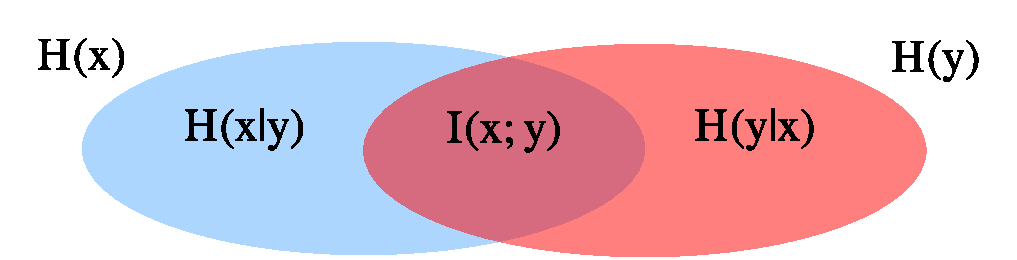
\includegraphics{figures/mutualinformation.pdf}
%\end{figure}

% \framebreak

% Mutual information can be used to perform \textbf{feature selection}. Quite simply, each variable $X_i$ is rated according to $I(X_i;Y)$: The more information we gain on $Y$ by observing $X_i$, the more "useful" $X_i$.

% \lz

% Let $\D = \Dset$ and $\D \{\cdot\}$ a subset of $\D$ for which condition $\cdot$ is fulfilled. Then, \textbf{information gain} is defined as:

% \footnotesize
% \begin{equation*}
% \begin{aligned}
% IG(\D, s) &= I(X_s;Y) \\
% &= H(Y) - H(Y|X_s) \\
% &= - \sum_{y \in Y} p(y) \log_2 p(y) + \sum_{x \in X_s} \sum_{y \in Y} p(x,y) \log_2 p(y|x) \\
% &= - \sum_{y \in Y} \frac{|\D\{Y = y\}|}{|\D|} \log_2 \sum_{y \in Y} \frac{|\D\{Y = y\}|}{|\D|} \\ &+
% \sum_{x \in X_s} \sum_{y \in Y} \frac{|\D\{Y = y, X_s = x\}|}{|\D|} \log_2 \frac{|\D\{Y = y, X_s = x\}|}{|\D\{X_s = x\}|}.
% \end{aligned}
% \end{equation*}
% \normalsize

% \framebreak

\begin{itemize}
  % \item Intuitively, mutual information quantifies the amount of shared information between variables.
  \item MI is a measure of the amount of "dependence" between variables. It is zero if and only if the variables are independent.
  \item On the other hand, if one of the variables is a deterministic function of the other, the mutual information is maximal, i.e. entropy of the first.
 \item Unlike (Pearson) correlation, mutual information is not limited to real-valued random variables.
    \item Mutual information can be used to perform \textbf{feature selection}. Quite simply, each variable $X_i$ is rated according to $I(X_i;Y)$, this is sometime called information gain.
  \item The same principle can also used in decision trees to select a feature to split on. Splitting on MI/IG is then equivalent to risk reduction with log-loss. 
\end{itemize}
\end{vbframe}
 

\begin{vbframe} {Mutual information vs. correlation}
  
  \begin{itemize}
    \item If two variables are independent, their correlation is 0.
    \item However, the reverse is not necessarily true. It is possible for two dependent variables to have 0 correlation because correlation only measures linear dependence.
    
\begin{center}
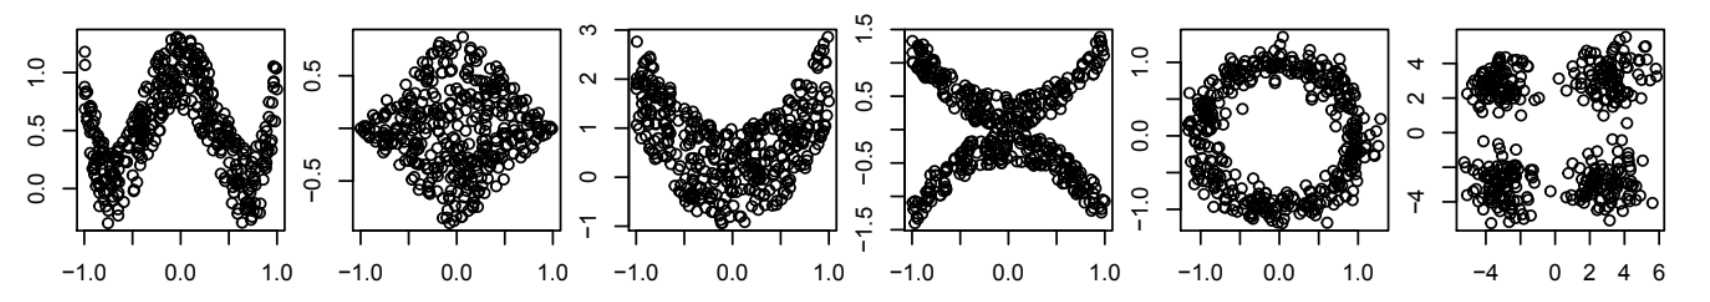
\includegraphics[width = 10cm ]{figure_man/correlation.png} \\
\end{center}

    \item The figure above shows various scatterplots where, in each case, the correlation is 0 even though the two variables are strongly dependent, and MI is large. 
    \item Mutual information can therefore be seen as a more general measure of dependence between variables than correlation.
  \end{itemize}

\end{vbframe}

\begin{vbframe} {Mutual information - example}

Let $X, Y$ be two correlated Gaussian random variables. $(X, Y) \sim \mathcal{N}(0, K)$ with correlation $\rho$ and covariance matrix $K$:

$$
K =
\begin{pmatrix}
  \sigma^2 & \rho \sigma^2 \\
  \rho \sigma^2 & \sigma^2
\end{pmatrix}
$$

Then $h(X) = h(Y) = \frac{1}{2} \log(2 \pi e) \sigma^2$, and $h(X,Y) = \log(2 \pi e)^2 |K| = \log(2 \pi e)^2 \sigma^4 (1 - \rho^2)$, and thus

\begin{equation*}
\begin{aligned}
I(X;Y) = h(X) + h(Y) - h(X,Y) = -  \frac{1}{2} \log(1 - \rho^2).
\end{aligned}
\end{equation*}

For $\rho = 0$, $X$ and $Y$ are independent and $I(X;Y) = 0$. \\
For $\rho = \pm 1$, $X$ and $Y$ are perfectly correlated and $I(X;Y) \rightarrow \infty$. 
\end{vbframe}

% \begin{vbframe} {Chain rule for information}


% $$I\left(X_{1}, X_{2}, \ldots, X_{n} ; Y\right)=\sumin I\left(X_{i} ; Y | X_{i-1}, X_{i-2}, \ldots, X_{1}\right)$$

% \textbf{Proof:$\quad$}
% \footnotesize
% \begin{equation*}
% \begin{aligned}
% I\left(X_{1}, X_{2}, \ldots, X_{n} ; Y\right) &= H\left(X_{1}, X_{2}, \ldots, X_{n}\right)-H\left(X_{1}, X_{2}, \ldots, X_{n} | Y\right) \\
% &=\sumin H\left(X_{i} | X_{i-1}, \ldots, X_{1}\right)-\sum_{i=1}^{n} H\left(X_{i} | X_{i-1}, \ldots, X_{1}, Y\right) \\
% &=\sumin I\left(X_{i} ; Y | X_{1}, X_{2}, \ldots, X_{i-1}\right).  
% \end{aligned}
% \end{equation*}

% \normalsize

% \end{vbframe}


% \begin{vbframe} {Chain rule for KL distance}

% \begin{equation*}
% \begin{aligned}
% D_{KL}(p(x, y) \| q(x,y)) &= D_{KL}(p(x) \| q(x)) + D_{KL}(p(y|x) \| q(y|x))
% \end{aligned}
% \end{equation*}

% \textbf{Proof:}

% \footnotesize

% \begin{equation*}
% \begin{aligned}
% D_{KL}(p(x, y) \| q(x,y)) &= \sum_x \sum_y p(x,y) \log \frac{p(x,y)}{q(x,y)} \\
% &= \sum_x \sum_y p(x,y) \log \frac{p(x)p(y|x)}{q(x)q(y|x)} \\
% &= \sum_x \sum_y p(x,y) \log \frac{p(x)}{q(x)} + \sum_x \sum_y p(x,y) \log \frac{p(y|x)}{q(y|x)} \\
% &= D_{KL}(p(x) \| q(x)) + D_{KL}(p(y|x) \| q(y|x))
% \end{aligned}
% \end{equation*}

% \normalsize


% \end{vbframe}


%old slide about KLD 
% %\normalsize
% The mutual information between two variables $X$ and $Y$ is also the KL divergence of the product of the marginal distributions $p_x(x) p_y(y)$ from the joint distribution $p(x,y)$ :
% % $I(x;y)$ is the \emph{information gain} achieved if the the joint distribution $p_{xy}(x,y)$ is used instead of the product of marginal distributions :
% 
% \begin{eqnarray*}
% I(X;Y) &\overset{(*)}{=}& D_{KL}(p_{xy}||p_x p_y) = \sum_{x \in \Xspace} \sum_{y \in \Yspace} p_{xy}(x, y) \cdot \log \biggl(\frac{p_{xy}(x, y)}{p_x(x)p_y(y)}\biggr)
% \end{eqnarray*}
% 
% For continuous random variables $X$ and $Y$ with joint density $p(x,y)$ and marginal densities $p_x(x) p_y(y)$, the mutual information is:
% 
% \begin{eqnarray*}
% I(X;Y) &=& D_{KL}(p_{xy}||p_x p_y) = \int_{x \in \Xspace} \int_{y \in \Yspace} p_{xy}(x, y) \cdot \log \biggl(\frac{p_{xy}(x, y)}{p_x(x)p_y(y)}\biggr)
% \end{eqnarray*}
% 
% 
% (Note: If $X$ and $Y$ are independent, $p(x,y)=p_x(x) p_y(y)$ and $I(X;Y)$ is zero.)
% \framebreak
% 
% (*) Derivation:
% 
% \footnotesize
% 
% 
% \begin{eqnarray*}
% I(X;Y) &=& H(Y) + H(X) - H(X, Y)\\
% &=& -\sum_{y \in \Yspace} p_y(y) \log_2(p_y(y)) -\sum_{x \in \Xspace} p_x(x) \log_2(p_x(x)) \\
% && -\sum_{x \in \Xspace, y \in \Yspace} p_{xy}(x, y) \log_2(p_{xy}(x, y))\\
% &=& -\sum_{x \in \Xspace, y \in \Yspace}p_{xy}(x, y) \log_2(p_y(y)) -\sum_{x \in \Xspace, y \in \Yspace} p_{xy}(x, y) \log_2(p_x(x)) \\
% && \quad+ \sum_{x \in \Xspace, y \in \Yspace} p_{xy}(x, y) \log_2(p_{xy}(x, y)) \\
% &=& \sum_{x \in \Xspace} \sum_{y \in \Yspace} p_{xy}(x, y) \cdot \log_2 \biggl(\frac{p_{xy}(x, y)}{p_x(x)p_y(y)}\biggr) = D_{KL}(p_{xy}||p_x p_y)
% \end{eqnarray*}
% 
% 




















% \begin{vbframe} {Summary}

% \begin{figure}
%     \centering
%       \scalebox{0.75}{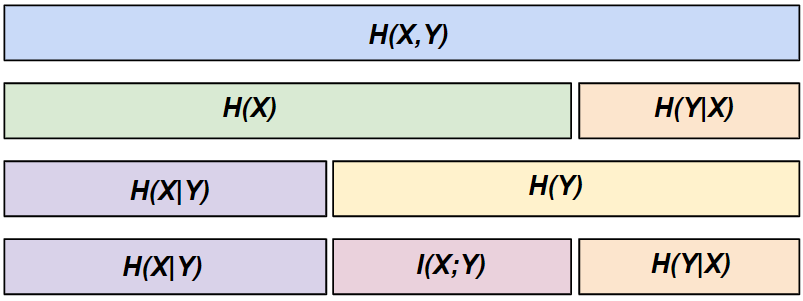
\includegraphics{figures/quants.png}}
% \end{figure}
  

%     \begin{align*}
%       H(X,Y) &= H(X) + H(Y|X) \\
%              &= H(Y) + H(X|Y)
%     \end{align*}
    
%     \begin{align*}
%       I(X;Y) &= H(X) - H(X|Y) \\
%              &= H(Y) - H(Y|X)
%     \end{align*}

% \end{vbframe}


%%%%%%%%%%%%%%%%%%%%%%%%%%%%%%%%%%%%%%%%%%%%%%%%%%%%%%%%%%%%%%%%%%
%%%%%%%%%%%%%%%%%%%%%%%%%%%%%%%%%%%%%%%%%%%%%%%%%%%%%%%%%%%%%%%%%%
%%%%%%%%%%%%%%%%%%          REFERENCES          %%%%%%%%%%%%%%%%%%
%%%%%%%%%%%%%%%%%%%%%%%%%%%%%%%%%%%%%%%%%%%%%%%%%%%%%%%%%%%%%%%%%%
% \begin{vbframe}
% \frametitle{References}
% \footnotesize{
% \begin{thebibliography}{99}
% 
% %%%%%%%%%%%%%%%%%%%%%%%%%%%%%%%%%%
% \bibitem[Chris Olah, 2015]{1} Chris Olah (2015)
% \newblock Visual Information Theory
% \newblock \emph{\url{http://colah.github.io/posts/2015-09-Visual-Information/}}
% %%%%%%%%%%%%%%%%%%%%%%%%%%%%%%%%%%
% \bibitem[Massimiliano Tomassoli, 2016]{2} Massimiliano Tomassoli (2016)
% \newblock Information Theory for Machine Learning
% \newblock \emph{\url{https://github.com/mtomassoli/papers/blob/master/inftheory.pdf}}
% %%%%%%%%%%%%%%%%%%%%%%%%%%%%%%%%%%
% \bibitem[Will Kurt, 2017]{3} Will Kurt, (2017)
% \newblock Kullback-Leibler Divergence Explained
% \newblock \emph{\url{https://www.countbayesie.com/blog/2017/5/9/kullback-leibler-divergence-explained}}
% %%%%%%%%%%%%%%%%%%%%%%%%%%%%%%%%%%
% \bibitem[Eric Jang, 2016]{4} Eric Jang, (2016)
% \newblock A Beginner's Guide to Variational Methods: Mean-Field Approximation
% \newblock \emph{\url{https://blog.evjang.com/2016/08/variational-bayes.html}}
% 
% \end{thebibliography}
% }
% \end{vbframe}

% \section{Information Theory and Machine Learning}

% \begin{vbframe} {KL to CE to LL}
% 
% \begin{equation*}
%   \begin{split}
%     \theta^* & = \argmin_{\theta} \sum_1^n KL (d_i \parallel f_{\theta}(x_i)) \\
%              & = \argmin_{\theta} \sum_1^n [H(d_i, f_{\theta}(x_i)) - H(d_i)] \\
%              & = \sum_1^n  H(d_i, f_{\theta}(x_i))
%   \end{split}
% \end{equation*}
% 
% \framebreak
% 
% \begin{equation*}
%   \begin{split}
%     \theta^* &= \argmin_{\theta} \sum_1^n \left( - \sum_y d_i(y) \log_2f_{\theta}(y|x_i) \right) \\
%              &= \argmin_{\theta} \sum_1^n (-\log_2f_{\theta}(y|x_i)) \\
%              &= \argmax_{\theta} \sum_1^n \log_2f_{\theta}(y|x_i) \\
%              &= \argmax_{\theta} \log \prod_1^n P(y_i|x_i;\theta) \\
%              &= \argmax_{\theta} \log P(y_1, \ldots , y_n | x_1, \ldots x_n ; \theta) \\
%              &= \argmax_{\theta} \log L(\theta)
%   \end{split}
% \end{equation*}
% 
% \end{vbframe}

% \begin{vbframe} {Density Estimation}
% 
% Minimizing the 
%   \begin{equation*}
%     \begin{split}
%       \theta^* &= \argmin_{\theta} KL(\hat{p} \parallel p_{\theta}) = \argmin_{\theta} [H(\hat{p},p_{\theta}) - H(\hat{p})] \\ &= \argmin_{\theta} H(\hat{p},p_{\theta}) = \argmin_{\theta} \E_{X \sim \hat{p}} [I_{p_{\theta}}(X)] \\
%                &= \argmin_{\theta} \sum_x \hat{p}(x) (- \log p_{\theta} (x)) \\
%                &= \argmax_{\theta} \sum_1^n \frac{1}{n} \log p_{\theta} (x_i) = \argmax_{\theta} \sum_1^n  \log p_{\theta} (x_i) \\
%                &= \argmax_{\theta} \log \prod_1^n p_{\theta} (x_i) = \argmax_{\theta} \log P(x_1, \ldots x_n | \theta) \\
%                &= \argmax_{\theta} \log L(\theta)
%     \end{split}
%   \end{equation*}
%   
% \end{vbframe}
% 
% \begin{vbframe} {Information Gain}
%   \begin{itemize}
%     \item Feature selection using information gain
%     \item Joint Mutual Information
%   \end{itemize}
% \end{vbframe}
% 
% \begin{vbframe} {Variational Inference}
% 
%   \begin{equation*}
%     \begin{split}
%       KL(q(z) \parallel p(z|x)) &= \E_q \left[ \log \frac {q(Z)} {p(Z|x)}  \right] \\
%                                 &= \E_q [\log q(Z)] - \E_q [\log p(Z|x)] \\
%                                 &= \E_q [\log q(Z)] - \E_q [\log p(Z,x)] + \log p(x) \\
%                                 &= -(\E_q [\log p(Z,x) - \E_q [\log q(Z)]) + \log p(x) \\
%                                 &= -L + \log p(x) 
%     \end{split}
%   \end{equation*}
%   where L is the ELBO (Evidence Lower Bound)
% \end{vbframe}

%\begin{vbframe} {Chain rule for entropy}
%\begin{columns}[T,onlytextwidth]
%\column{0.3\textwidth}
%\textbf{Example: Consider a node in a decision tree with 7 samples that belong to either the $+$ or the $-$ class.} \\
%\lz
%\begin{center}
%<<entropy-ex1, echo=FALSE, size = "footnotesize">>=
%library(knitr)
%ex1 <- cbind(class=c("+","+","-","+","-","-", "-"), attr_1 = c(T,T,T,F,F,F,F), attr_2 = c(T,T,F,F,T,T,T))
%kable(ex1)
%@
%\end{center}
%\column{0.65\textwidth}
%\begin{itemize}
%\item How big is the uncertainty/entropy in \textit{class} (in bits)?
%%\small
%\begin{eqnarray*}
%H(\text{class}) &=& - \sum_{k=+,\, -} p(k) \log_2(p(k)) \\
%&=& - \frac{3}{7} \log_2\left(\frac{3}{7}\right)  - \frac{4}{7} \log_2\left(\frac{4}{7}\right) \\
%&=& 0.985
%\end{eqnarray*}
%%\normalsize
%\item How much can it be reduced by knowing the other attributes?
%\end{itemize}
%\end{columns}


%\framebreak
%\begin{columns}[T,onlytextwidth]
%\column{0.3\textwidth}
%\textbf{Example:} \\
%\lz
%\begin{center}
%<<entropy-ex2, echo=FALSE, size = "footnotesize">>=
%library(knitr)
%kable(ex1)
%@
%\end{center}
%\column{0.65\textwidth}
%\scriptsize

%\vspace*{1.5cm}

%$H(\text{class}|\text{attr}_1 = T) = - \frac{2}{3} \log_2(\frac{2}{3}) - \frac{1}{3} \log_2(\frac{1}{3}) = 0.92$ \\
%$H(\text{class}|\text{attr}_1 = F) = - \frac{1}{4} \log_2(\frac{1}{4}) - \frac{3}{4} \log_2(\frac{3}{4}) = 0.81$ \\
%$H(\text{class}|\text{attr}_2 = T) = - \frac{2}{5} \log_2(\frac{2}{5}) - \frac{3}{5} \log_2(\frac{3}{5}) = 0.97$ \\
%$H(\text{class}|\text{attr}_2 = F) = - \frac{1}{2} \log_2(\frac{1}{2}) - \frac{1}{2} \log_2(\frac{1}{2}) = 1$ \\
%\lz
%$H(\text{class}|\text{attr}_1) = \frac{3}{7} 0.92 + \frac{4}{7} 0.81 = 0.86$ \\
%$H(\text{class}|\text{attr}_2) = \frac{5}{7} 0.97 + \frac{2}{7} 1 = 0.98$

%\normalsize

%\end{columns}

%\lz

%By further splitting the node using either of the attributes, the uncertainty in class is reduced.

%\framebreak

%\begin{columns}[T,onlytextwidth]
%\column{0.3\textwidth}
%\textbf{Example:} \\
%\lz
%\begin{center}
%<<entropy-ex3, echo=FALSE, size = "footnotesize">>=
%library(knitr)
%kable(ex1)
%@
%\end{center}
%\column{0.65\textwidth}
%\begin{itemize}
%\item The reduction in uncertainty, or equivalently, gain in information is:
%\footnotesize
%\begin{eqnarray*}
%H(\text{class}) - H(\text{class}|\text{attr}_1) &=& 0.985 - 0.86 \\
% &=& 0.125
%\end{eqnarray*}

%\begin{eqnarray*}
%H(\text{class}) - H(\text{class}|\text{attr}_2) &=&  0.985 - 0.98 \\
%&=& 0.005
%\end{eqnarray*}
%% \normalsize
%% \lz
%\item $\text{attr}_1$ tells us more about $\text{class}$. Therefore, to improve the predictive performance of the decision tree in the CART algorithm, it is better to further split the node using $\text{attr}_1$, rather than $\text{attr}_2$.
%\end{itemize}

%\end{columns}

%\end{vbframe}

\endlecture
\end{document}



